\chapter{Methods}

% to complete!!

In a double difference evaluation, the first step is to assign sampling units to treatment and control groups based on given measurable criteria. After sampling units have been assigned to treatment and control groups, the control group serves as a valid counterfactual for the treatment group if and only if one can establish parallel trends between the treatment and control group on the outcome variables of interest. Satisfying the assumption of parallel trends is how one ensures internal validity in a double difference evaluation and what ensures that the  double difference estimator serves as an unbiased estimate of the average treatment effect.\\

The measurable criteria used in this study was a district-level Flood Risk Index calculated using remotely-sensed flood frequency and flood impact information. Flood risk was used to group districts into treatment and control groups based on the study hypothesis, which details why the benefits of the FIS might be most salient in flood-prone districts relative to non flood-prone districts. The steps to estimate impact were as follows:

\begin{enumerate}
  \item Develop a Flood Risk Index.
  \item Threshold the Flood Risk Index.
  \item Examine parallel trends between treatment and control groups on the outcome variables.
\end{enumerate}

Each step is detailed below.

\section{Develop a Flood Risk Index}

Measuring flood risk is a complex process; it involves accounting for not only a given region’s flood frequency but also the region’s social and economic vulnerability. If a given region has many low-rise buildings or farmable land on it, for example, it is at higher flood risk than a comparable region without those assets on it. It is possible to capture both important dimensions of flood risk using two types of geospatial information: flood recurrence intervals, and the location of various assets of interest (e.g. people, cropland, roads). The intersection of these two types of flood information for various intervals of time provides a more complete measure of flood risk that is based not only on flood frequency, but the overall historical flood impact as well. The flood risk index calculation methodology is as follows:

\begin{enumerate}
  \item Compute the average number of flood-affected people per year per district.
  \item Compute the average area of flood-affected cropland per year per district.
  \item Convert the average area of flood-affected cropland per year per district into average numbers of flood-affected people per year per district.
  \item Sum the values from Steps 1 and 3 to calculate the raw Flood Risk Index.
  \item Use a z-score conversion to normalize the raw Flood Risk Index values.
\end{enumerate}

Each of these steps is detailed further below.

\subsection{Compute the average number of flood-affected people per year per district.}

Given that recurrence intervals can be thought of as different flood frequency scenarios, we can use the data from Table 6.2 to calculate the average number of flood-affected people overall flood frequency scenarios. We can do this by calculating the marginal number of flood-affected people under each scenario:

\[ MI_T = (I_T - I_{T-1}) / T \]

Where (\({MI_T}\)) is the marginal impact under recurrence interval (\({T}\)). The term (\({I_T}\)) represents the total impact (i.e. total number of flood-affected people) and (\(I_{T-1}\)) represents the same for the prior recurrence interval. Table 8.1 uses the values from Table 6.2 to calculate the marginal impact under each recurrence interval for the Ada East district. Table 8.1 illustrates how one would implement the equation on the last page to calculates the marginal population impact for each district across all five recurrence intervals.\\

Finally, we can calculate the average impact across all flood frequency scenarios by applying a weighted sum, like so:

\[ I_{\mu} = \sum_{T=1}^{5} MI_T * w_T \]

In this equation, the left-hand term refers to the average population impact or the average cropland impact in a given district across all flood recurrence intervals. The term \({MI_T}\) represents the marginal impact in a given recurrence interval \({T}\). The term \({w_T}\) represents the weight for a given recurrence interval as shown in Table 8.2. Weights provided in Table 8.2 correspond roughly to the recurrence interval's annual exceedance probability (e.g. 2-Year Recurrence Interval corresponds to a 50 percent probability of occurrence, 5-Year Recurrence Interval corresponds to a 20 percent probability of occurrence, and so on). All weights in Table 8.2 sum to 1.00.\\

Table 8.3 provides an example of how the formula from the prior page, used to calculate average impact, is implemented. As shown in Table 8.3, the computed population impact for the Ada East district is 5.36231. This computed average is a measure of both flood frequency and impact severity. It measures not only the frequency of flooding in a given region, but the total number of people that would be affected if that region were to actually flood in the following year. \\

\begin{table}
\centering
\begin{tabular}{|p{3cm}|c|c|}
\hline
\textbf{Interval (\({T}\))} & \textbf{District} & \textbf{Marginal Population Impact}\\
\hline
2-Year Interval\rule{0pt}{4ex} & Ada East & (0 - 0) / 2 = 0 \\
5-Year Interval\rule{0pt}{4ex} & Ada East & (80 - 0) / 5 = 16 \\
10-Year Interval\rule{0pt}{4ex} & Ada East & (230 - 80) / 10 = 15\\
15-Year Interval\rule{0pt}{4ex} & Ada East & (328 - 230) / 15 = 6.533\\
20-Year Interval\rule{0pt}{4ex} & Ada East & (410 - 328) / 20 = 4.1\\
\hline
\end{tabular}
\caption{Marginal population impact for Ada East}
\end{table}

\begin{table}
\centering
\begin{tabular}{|c|c|}
\hline
\textbf{Recurrence Interval (\({T}\))} & \textbf{Weight (\({w_T}\))}\\
\hline
2-Year Interval\rule{0pt}{4ex} & 0.580 \\
5-Year Interval\rule{0pt}{4ex} & 0.200 \\
10-Year Interval\rule{0pt}{4ex} & 0.100 \\
15-Year Interval\rule{0pt}{4ex} & 0.07 \\
20-Year Interval\rule{0pt}{4ex} & 0.05 \\
\hline
\end{tabular}
\caption{Weights for each Recurrence Interval}
\end{table}

\begin{table}
\centering
\begin{tabular}{|p{4cm}|p{7cm}|}
\hline
\textbf{Metric} & \textbf{Formula}\\
\hline
Avg Flood-Affected Population (\({I_P}\)) & (0 * 0.58) + (16 * 0.20) + (15 * 0.10) + (6.533 * 0.07) + (4.1 * 0.05) = 5.36231\\
\hline
\end{tabular}
\caption{Average Population Impact for Ada East}
\end{table}

We now repeat this step using cropland data, and calculate the average hectares of flood-affected cropland per district.

\subsection{Compute the average area of flood-affected cropland per year per district.}

\begin{table}
\centering
\begin{tabular}{|p{3.5cm}|p{4.5cm}|p{4.5cm}|}
\hline
\textbf{District} & \textbf{Avg Flood-Affected Population (\({I_P}\))} & \textbf{Avg Flood-Affected Cropland}\\
\hline
Accra Metropolis\rule{0pt}{4ex} & 30.744500 & 0.000025\\
Ada East\rule{0pt}{4ex} & 5.36231 & 0.214428\\
Ada West\rule{0pt}{4ex} & 23.737333 & 0.725215\\
Adaklu\rule{0pt}{4ex} & 0.000000 & 0.000772\\
\hline
\end{tabular}
\caption{Average overall annual flood impacts per district, inconsistent units of measurement}
\end{table}

Using the process outlined in Step 1, we calculate the average hectares of flood-affected cropland for each of Ghana's 216 districts. A sample of the full results of implementing this calculation is provided in Table 8.4. As shown in Table 8.4, the average overall annual flood impacts per district is simply a weighted sum of the marginal population impacts.

\subsection{Convert the average area of flood-affected cropland per year per district into average numbers of flood-affected people per year per district.}

We cannot yet add the values from Steps 1 and 2 together, because the two assets are not in the same unit of measurement. From Step 1, we see that the unit of the people-based asset is the number of flood-affected people per district. From Step 2, we see that the unit of the cropland-based asset is the area of flood-affected cropland per district.\\

To ensure these two assets are comparable, we can set an arbitrary conversion rate to convert the cropland-based asset into the people-based one (i.e. convert the average area of flood-affected cropland into an average number of flood-affected people). For the purposes of this study, the following conversion rate is used:

\[ 10{H} = 1{P} \]

In this equation, \({H}\) represents the hectares of flood-affected cropland, and \({P}\) represents the number of flood-affected people. The conversion rate used is 10 hectares of flood-affected cropland to 1 flood-affected person.\\

This conversion rate is logical as one could argue that, all things being equal, individual human lives are more valuable than crops. The damage that flooding does to a single human life (whether ‘damage’ refers to death, or less severe kinds of damage) is likely more costly to society than the damage that flooding does to a single hectare of cropland. In sum, this conversion rate was set arbitrarily based on the idea that, all things being equal, the cost to society of one flood-affected person is greater than the cost to society of one hectare of flood-affected cropland.

Using this conversion rate, the third column from Table 8.4 can divided by a factor of 10 and re-written as follows:

\begin{table}
\centering
\begin{tabular}{|c|c|c|}
\hline
\textbf{District} & \textbf{Population Impact \({I_P}\)} & \textbf{Cropland Impact (scaled) \({I_C}\)}\\
\hline
Accra Metropolis\rule{0pt}{4ex} & 30.744500 & 2.500000e-06\\
Ada East\rule{0pt}{4ex} & 5.364478 & 2.144283e-02\\
Ada West\rule{0pt}{4ex} & 23.744585 & 7.252150e-02\\
Adaklu\rule{0pt}{4ex} & 0.000008 & 7.716667e-05\\
\hline
\end{tabular}
\caption{Average overall annual flood impacts per district, consistent units of measurement}
\end{table}

Table 8.5 is identical to Table 8.4 except that the last column is now scaled by a factor of 100 so that the units of both impacts are now consistent.

\subsection{Sum the values from Steps 1 and 3 to calculate the raw Flood Risk Index.}

After calculating average overall annual flood impact in consistent units, we can now sum row-wise to arrive at a raw Flood Risk Index:

\[ FRI = I_P + I_C \]

In this formula, each type of critical asset is weighted equally. This is because both population and cropland are equally important in terms of impact severity.

\subsection{Use a z-score conversion to normalize the raw Flood Risk Index values.}

Finally, we convert the raw index values using z-scores to normalize the index range. The z-score conversion involves subtracting the mean of the distribution from each value, and dividing the quantity by the standard deviation of the distribution:

\[ z = ({FRI-\mu})/{\sigma} \]

Where \({z}\) represents the normalized Flood Risk Index, \({FRI}\) represents the raw Flood Risk Index value, and \({\mu}\) \({\sigma}\) represent the mean and standard deviation of the distribution of raw Flood Risk Index values. Table 8.6 applies the z-score normalization to compute the final Flood Risk Index (only a sample of the full data set is shown). \\

\begin{table}
\centering
\begin{tabular}{|c|c|c|}
\hline
\textbf{District} & \textbf{Raw Flood Risk Index (\({FRI}\))} & \textbf{Final Flood Risk Index (\({z}\))}\\
\hline
Accra Metropolis\rule{0pt}{4ex} & 30.744500 & 3.185309\\
Ada East\rule{0pt}{4ex} & 5.36231 & 0.384569\\
Ada West\rule{0pt}{4ex} & 23.737333 & 2.412853\\
Adaklu\rule{0pt}{4ex} & 0.000000 & -0.207412\\
\hline
\end{tabular}
\caption{Raw Flood Risk Index and final Flood Risk Index}
\end{table}

It is critical to note that this calculation methodology for the Flood Risk Index assumes that a district is at higher flood risk if and only if it contains either population or cropland-based assets on it that could be affected were that region to actually flood in the following year. If a region does not have any flood risk assets on it, it would rank on the bottom of the index. In this way, the index measures both flood frequency and impact severity. The spatial distribution of the Flood Risk Index across Ghana can be seen in the Figure 8.1.\\

\begin{figure}
  \begin{center}
    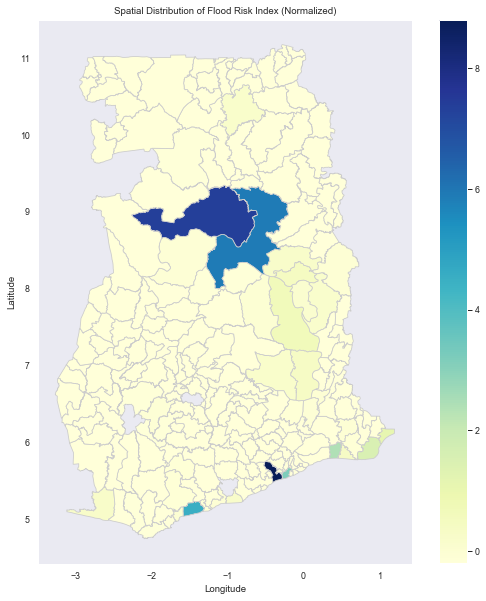
\includegraphics[scale=0.8]{images/01-map.png}
  \end{center}
  \caption{Spatial distribution of final Flood Risk Index}
\end{figure}

As shown in Figure 8.1, the flood-prone districts in Ghana are clustered in the northeast and western regions of the country. The non flood-prone districts of Ghana are all of the surrounding regions. Flood risk experts\footnote{Cloud to Street remote sensing scientists} agree that the map shown in Figure 8.1 above roughly corresponds to their expectations around both flood frequency and social and economic vulnerability. The frequency distribution of these values can be seen in Figure 8.2. \\

\begin{figure}
  \begin{center}
    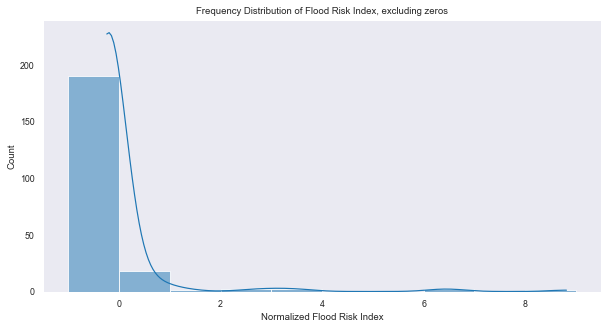
\includegraphics[scale=0.7]{images/02-graph.png}
  \end{center}
  \caption{Frequency distribution of final Flood Risk Index}
\end{figure}

Figure 8.2 illustrates the distribution of the normalized flood risk index values (i.e. the z-score conversion of the raw index values). Each bin of the histogram represents one standard deviation from the mean. From the frequency distribution, we can see that the vast majority of Ghana’s 216 districts fall within 1 standard deviation below the normalized mean of the Flood Risk Index. A small percentage of districts are severely high risk, falling anywhere from 3 to 8 standard deviations above the mean.

\section{Threshold the Flood Risk Index}

\begin{figure}
  \begin{center}
    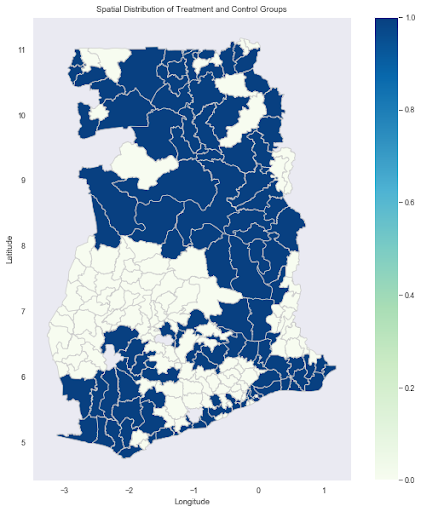
\includegraphics[scale=0.95]{images/03-map.png}
  \end{center}
  \caption{Spatial distribution of treatment-control boundary}
\end{figure}

After all of Ghana’s 216 districts were given a value on the normalized Flood Risk Index, a threshold was set to mark the point beyond which a given district would be labelled ‘flood-prone’ and thus placed into the Treatment Group. Because empirical methods could not be used to identify an appropriate threshold, the threshold was set arbitrarily following the expertise of remote sensing scientists familiar with the flood risk landscape in Ghana.\\

\begin{figure}
  \begin{center}
    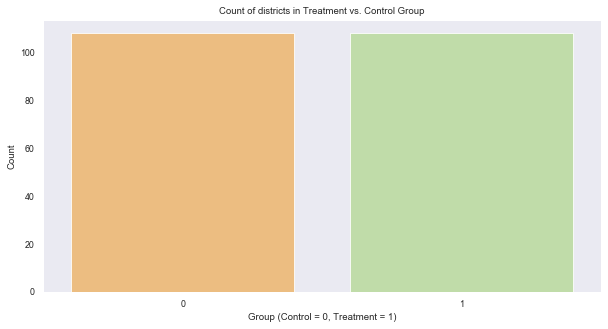
\includegraphics[scale=0.7]{images/04-graph.png}
  \end{center}
  \caption{Frequency distribution of treatment-control boundary}
\end{figure}

The threshold used was the 50th percentile. This meant that the 216 Ghanaian districts which ranked in the top 50 percent of the Flood Risk Index were grouped into Treatment, and all remaining districts (i.e. those in the bottom 50 percent) were grouped into Control. The spatial distribution of treatment and control groups can be seen in Figure 8.3. The map in Figure 8.3 illustrates the spatial distribution of the treatment-control assignment using the 50th percentile threshold. Using this threshold, treatment districts are classified as those in  mid and northern Ghana, as well as southwest Ghana. Control districts are all those surrounding these districts. \\

The number of districts in each group is illustrated in Figure 8.4. Because the threshold was set at the 50th percentile, exactly half of the 216 districts (108 districts) were binned in the treatment and control group each.

\section{Examine parallel trends between treatment and control groups on the outcome variables}

After grouping all of Ghana’s 216 districts into either Treatment or Control, the final step was to examine group means on observable characteristics to determine if there existed parallel trends. As mentioned in earlier sections of this paper, the validity of the Control group as a counterfactual for the Treatment group hinges on the existence of parallel trends between Treatment and Control Groups prior to the start of the program. \\

Parallel trends were examined on two outcome variables of interest:

\begin{itemize}
    \item The average number of total flood-affected people per district, and
    \item The average area of total flood-affected cropland per district.
\end{itemize}

Using line graphs, we are able to see visually that for the 35-year satellite record, parallel trends do not exist in the average number of total flood-affected people per district in the treatment versus control group. These visual trends are shown in Figure 8.5. \\

\begin{figure}
  \begin{center}
    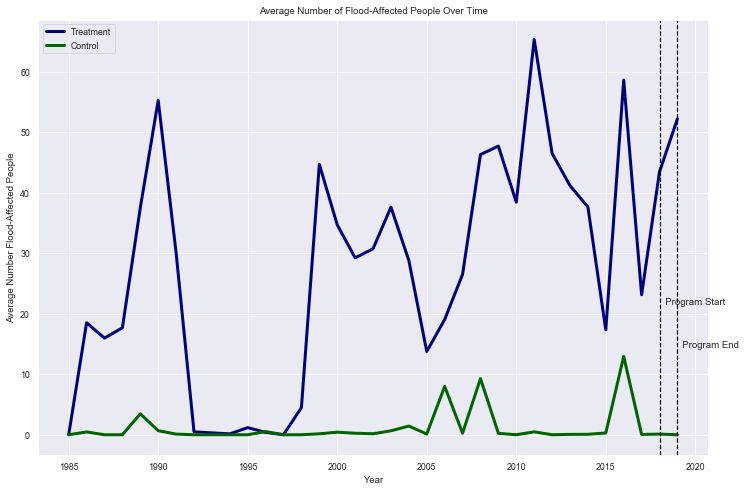
\includegraphics[scale=0.6]{images/05-parallel-trends-population.png}
  \end{center}
  \caption{Visualization of parallel trends test in total flood-affected population outcome variable.}
\end{figure}

\begin{figure}
  \begin{center}
    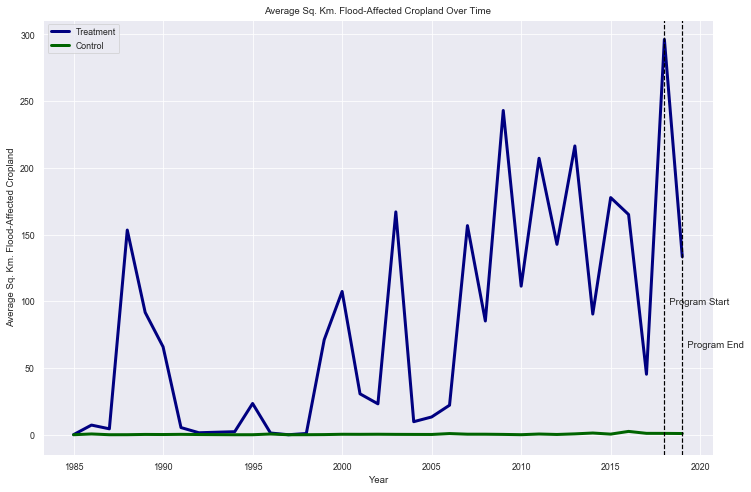
\includegraphics[scale=0.6]{images/06-parallel-trends-cropland.png}
  \end{center}
  \caption{Visualization of parallel trends test in total flood-affected cropland outcome variable.}
\end{figure}

The year-over-year change in the mean flood-affected population over the last 35 years in the satellite record shows a lack of parallel trends between treatment and control group means.

Parallel trends means that the lines in this line graph are parallel, where each line represents the group mean in a given year. When examining the treatment group on average flood-affected population overtime in Figure 8.5, we see that the lines are not parallel in all years prior to the year 2015. From 2015 to 2018, the lines are parallel. 2015 onward, the rates of change from one year to the next are in the correct direction (increase from 2015 to 2016, decrease from 2016 to 2017, and increase from 2017 to 2018). However, the rates of change are not consistent across Treatment and Control groups; in 2016 for example, there was an 1.7 percent increase in average flood affected population for the Treatment group but a 10.6 percent increase for the Control group. When examining the treatment group on average flood-affected cropland overtime in Figure 8.6, we see that the line exhibits a highly cyclical pattern. Meanwhile, the control group on this characteristic has a flat line. The lines are clearly not parallel to one another.

Mathematically, we can confirm this visual pattern of a lack of parallel trends by calculating the slope of the line between each year on the x-axis, using point-slope form:

\[ {m} = ({x_1 - x_2}) / ({y_1 - y_2}) \]

The data shown in Figure 8.5 was used to calculate the slope of each line to mathematically confirm that we do not observe parallel trends. As shown in Figure 8.5 the x-axis pertain to a given year, and the y-axis pertains to the average number of flood affected people in the given year. \\

Thus, (\({x_1 - x_2}\)) pertains to the change in number of years, and (\({y_1 - y_2}\)) pertains to the change in average number of flood-affected people over those number of years. The complete list of slope calculations can be found in Appendix 12.1: Mathematical confirmation of a lack of parallel trends. \\

The lack of parallel trends across these two outcome variables indicates the presence of selection bias in the treatment and control group assignment. This means that using the Flood Risk Index in its current form as the group assignment variable does not allow the control group to serve as a valid counterfactual for the treatment group. Running a double difference estimation on these groups would ultimately not produce an unbiased estimate of the average treatment effect. Several extraneous factors could explain any observed differences in the treatment and control group on food security outcome variables of interest.

